\immediate\write18{tex tikzmark.dtx}
\documentclass[a4paper]{article}
\usepackage{amsmath}
\usepackage{tikz}
\usepackage{lipsum}
\usepackage{listings}
\usetikzlibrary{arrows,tikzmark,fit,shadows}
\usetikzmarklibrary{%
%  highlight,
  listings
}

\newcommand{\tikzmarkset}[2]{
	\pgfkeys{/tikz/#1/.cd,#2}
}

\begin{document}

hello\tikzmark{a} world


\begin{tikzpicture}[remember picture, overlay]
\draw (0,0) -- (1,-1);
\draw[->] (0,0) to[bend left] (pic cs:a);
\end{tikzpicture}

\begin{tikzpicture}[remember picture, overlay, shift={(1cm,-1cm)}, scale=2]
\draw (0,0) -- (1,-1);
\draw[->] (0,0) to[bend left] (pic cs:a);
\end{tikzpicture}

\end{document}


\[\highlight[colour=green!50]{x+y}=100\]

\tikzmarkset{highlighter}{left margin=1ex,right margin=1ex, top margin=3ex, bottom margin=4ex,colour=cyan!50}
\[\highlight{x+y}=100\] % same as before? Strange!

\tikzmarkset{highlighter}{colour=orange!50,initial offset=1pt,final offset=1pt}
\[\highlight[final depth=7pt]{x+y}=100\]

\tikzset{/tikz/highlighter/.cd,colour=green!50}
\[\highlight[initial offset=1pt, final offset=1pt,height=14pt, final depth=11pt]{\dfrac{x}{y}}=100\]

% check if holds many times
\tikzmarkset{highlighter}{colour=white!20!violet!80!purple,initial offset=1pt,final offset=1pt,height=16pt, final depth=11pt}
\begin{equation}
V(z)=\sum_{\kappa=0}^{\infty}{\; \highlight{\int_{0}^{\infty}{\dfrac{\mathrm{e}^{-\lambda x}\cdot (\lambda x)^\kappa}{\kappa!} \, b(x)\,\mathrm{d} x}}\cdot z^\kappa}
\end{equation}

\begin{equation}
V(z)=\sum_{\kappa=0}^{\infty}{\; \highlight{\int_{0}^{\infty}{\dfrac{\mathrm{e}^{-\lambda x}\cdot (\lambda x)^\kappa}{\kappa!} \, b(x)\,\mathrm{d} x}}\cdot z^\kappa}
\end{equation}

\[\highlight{\dfrac{x}{y}}=100\]

\[\highlight[initial offset=1pt, final offset=1pt, final depth=5pt]{x+y}=100\] % it inheriths the height
\[\highlight[initial offset=1pt, final offset=1pt, height=8pt, final depth=5pt]{x+y}=100\] % custom height

\tikzmarkset{fader}{colour=white!20!violet!80!purple,opacity=0.3,cap=rect} % cap don't seem to work
\begin{equation}
V(z)=\sum_{\kappa=0}^{\infty}{\; \fade{\int_{0}^{\infty}{\dfrac{\mathrm{e}^{-\lambda x}\cdot (\lambda x)^\kappa}{\kappa!} \, b(x)\,\mathrm{d} x}}\cdot z^\kappa}
\end{equation}


\tikzset{
  next page=below,
  fader/colour=gray,
  fader/opacity=.8,
%  every highlighter/.style={rounded corners},
  line/.style={
    draw,
    rounded corners=3pt,
    -latex
  },
  balloon/.style={
    draw,
    fill=blue!20,
    opacity=0.4,
    inner sep=4pt,
    rounded corners=2pt
  },
  comment/.style={
    draw,
    fill=blue!70,
    text=white,
%    text width=3cm,
%    minimum height=1cm,
    rounded corners,
    drop shadow,
    align=left,
%    font=\scriptsize
  },
}

\newcommand\balloon[4]{%
  \pgfmathtruncatemacro\firstline{%
    #3-1
  }%
  \iftikzmark{line-#2-\firstline-start}{%
    \iftikzmark{line-#2-#3-first}{%
      \xdef\blines{({pic cs:line-#2-\firstline-start} -| {pic           cs:line-#2-#3-first})}%
    }{%
      \iftikzmark{line-#2-#3-start}{%
        \xdef\blines{({pic cs:line-#2-\firstline-start} -| {pic             cs:line-#2-#3-start})}%
      }{%
        \xdef\blines{(pic cs:line-#2-\firstline-start)}%
      }%
    }%
  }{%
    \xdef\blines{}%
  }%
  \foreach \k in {#3,...,#4} {%
    \iftikzmark{line-#2-\k-first}{%
      \xdef\blines{\blines (pic cs:line-#2-\k-first) }
    }{}
    \iftikzmark{line-#2-\k-end}{%
      \xdef\blines{\blines (pic cs:line-#2-\k-end) }
    }{}
  }%
  \ifx\blines\empty
  \else
  \edef\temp{\noexpand\tikz[remember picture,overlay]\noexpand\node[fit={\blines},balloon] (#1) {};}%
\temp
  \fi
}

\makeatletter
\def\hl@debug@draw#1#2#3#4{%
    \begin{tikzpicture}[
      remember picture,
      overlay,
      baseline=0pt,
      /tikz/highlighter/.cd,
      #1,
      /tikz/.cd,
      highlight=#2,
      every path/.append style={
        highlight=#2,
        thick,
        black,
      }
    ]%
    \tikz@scan@one@point\pgfutil@firstofone(#3)\relax
    \pgf@ya=\pgf@y
    \tikz@scan@one@point\pgfutil@firstofone(#4)\relax
    \pgf@yb=\pgf@y
    \ifdim\pgf@ya=\pgf@yb
    \draw[->] (#3) -- ++(-1*\pgfkeysvalueof{/tikz/highlighter/initial offset},\pgfkeysvalueof{/tikz/highlighter/initial height}) coordinate (start);
    \draw[->] (#4) -- ++(\pgfkeysvalueof{/tikz/highlighter/final offset},-1*\pgfkeysvalueof{/tikz/highlighter/final depth}) coordinate (end);
    \draw[dashed] (start) rectangle (end);
    \else
    \page@node
    \path (page.east) ++(\pgfkeysvalueof{/tikz/highlighter/right margin},0pt) coordinate (east);
    \path (page.west) ++(-1*\pgfkeysvalueof{/tikz/highlighter/left margin},0pt) coordinate (west);
  \pgfmathsetlength\pgf@x{\pgfkeysvalueof{/tikz/highlighter/initial height}}%
    \advance\pgf@yb by \pgf@x\relax
  \pgfmathsetlength\pgf@x{-1*\pgfkeysvalueof{/tikz/highlighter/final depth}}%
    \advance\pgf@ya by \pgf@x\relax
    \ifdim\pgf@yb>\pgf@ya
    \draw[->] (#3) -- ++(-1*\pgfkeysvalueof{/tikz/highlighter/initial offset},\pgfkeysvalueof{/tikz/highlighter/initial height}) coordinate (start);
    \draw[->] (#3) -- ++(0pt,-1*\pgfkeysvalueof{/tikz/highlighter/final depth}) coordinate (end);
    \draw[dashed] (start) rectangle (end -| east);
\draw[->] ([yshift=5pt]end -| page.east) -- ([yshift=5pt]end -| east);
    \draw[->] (#4) -- ++(0pt,\pgfkeysvalueof{/tikz/highlighter/initial height}) coordinate (start);
    \draw[->] (#4) -- ++(\pgfkeysvalueof{/tikz/highlighter/final offset},-1*\pgfkeysvalueof{/tikz/highlighter/final depth}) coordinate (end);
    \draw[dashed] (start -| west) rectangle (end);
\draw[->] ([yshift=-5pt]start -| page.west) -- ([yshift=-5pt]start -| west);
    \else
    \draw[->] (#3) -- ++(-1*\pgfkeysvalueof{/tikz/highlighter/initial offset},-1*\pgfkeysvalueof{/tikz/highlighter/initial depth}) coordinate (start);
    \draw[->] (#4) -- ++(\pgfkeysvalueof{/tikz/highlighter/final offset},-1*\pgfkeysvalueof{/tikz/highlighter/final depth}) coordinate (end);
    \draw[->] (#3) -- ++(-1*\pgfkeysvalueof{/tikz/highlighter/initial offset},\pgfkeysvalueof{/tikz/highlighter/initial height}) coordinate (tl);
    \draw[->] (#4) -- ++(\pgfkeysvalueof{/tikz/highlighter/final offset},\pgfkeysvalueof{/tikz/highlighter/final height}) coordinate (mr);
\draw[->] ([yshift=-5pt]tl -| page.east) -- ([yshift=-5pt]tl -| east);
\draw[->] ([yshift=-5pt]start -| page.west) -- ([yshift=-5pt]start -| west);
    \draw[dashed] (start) -- (tl) -- (tl -| east) -- (mr -| east) -- (mr) -- (end) -- (end -| west) -- (start -| west) -- cycle;
    \fi
    \fi
    \end{tikzpicture}}

\let\hl@orig@draw=\hl@draw

\tikzset{
  highlighter/debug/.is choice,
  highlighter/debug/.default=on,
  highlighter/debug/on/.code={\let\hl@draw=\hl@debug@draw},
  highlighter/debug/off/.code={\let\hl@draw=\hl@orig@draw},
}

\makeatother

\newcommand{\tikzmarkhighlightset}[1]{
	\pgfkeys{/tikz/highlighter/.cd,#1}
}

\newcommand{\tikzmarkfadeset}[1]{
	\pgfkeys{/tikz/fader/.cd,#1}
}

\def\testtext{%
The sun was shining on the sea, shining with all its might.
\hlstart
And this was very odd because it was the middle of the night.
\hlend
The moon was up there sulkily because she thought the sun had no
business to be there after the day was done.
\hlstart
``It's very rude of him,'' she said, ``to come and spoil the fun.''
\hlend

\noindent The sun was shining on the sea, shining with all its might.
And this was very odd because it was the middle of the night.
\hlstart
The moon was up there sulkily because she thought the sun had no business to be there after the day was done\hlend.
``It's very rude of him,'' she said, ``to come and spoil the fun.''
}

\section{Highlighting}

\testtext

\subsection{The Expansion Parameters}

\subsubsection{Defaults}

\tikzset{highlighter/debug=off}

\testtext

\tikzset{highlighter/debug}

\testtext

\subsubsection{All Zero}

\tikzmarkhighlightset{
  initial height=0pt,
  initial offset=0pt,
  initial depth=0pt,
  final height=0pt,
  final offset=0pt,
  final depth=0pt,
  left margin=0pt,
  right margin=0pt,
}

\tikzset{highlighter/debug=off}

\testtext

\tikzset{highlighter/debug}

\testtext

\subsubsection{All Positive}

\tikzmarkhighlightset{
  initial height=10pt,
  initial offset=10pt,
  initial depth=10pt,
  final height=10pt,
  final offset=10pt,
  final depth=10pt,
  left margin=10pt,
  right margin=10pt,
}
\tikzset{highlighter/debug=off}

\testtext

\tikzset{highlighter/debug}

\testtext

\subsubsection{All Negative}

\tikzmarkhighlightset{
  initial height=-10pt,
  initial offset=-10pt,
  initial depth=-10pt,
  final height=-10pt,
  final offset=-10pt,
  final depth=-10pt,
  left margin=-10pt,
  right margin=-10pt,
}

\tikzset{highlighter/debug=off}

\testtext

\tikzset{highlighter/debug}

\testtext

\tikzset{highlighter/debug=off}

\newpage

\tikzmarkhighlightset{
  initial height=\baselineskip,
  initial depth=.5ex,
  initial offset=.5\baselineskip,
  final height=\baselineskip,
  final depth=.5ex,
  final offset=.5\baselineskip,
  left margin=.5\baselineskip,
  right margin=.5\baselineskip,
  top margin=.5\baselineskip,
  bottom margin=-.5\baselineskip,
}

\vlstart The sun was shining on the sea, shining with all its might.
And this was very odd because it was the middle of the night.
The moon was up there sulkily because she thought the sun had no
business to be there after the day was done.
``It's very rude of him,'' she said, ``to come and spoil the fun.''

\vlend The sun was shining on the sea, shining with all its might.
And this was very odd because it was the middle of the night.
The moon was up there sulkily because she thought the sun had no
business to be there after the day was done.
``It's very rude of him,'' she said, ``to come and spoil the fun.''


The sun was shining on the sea, \vlstart shining with all its might.
And this was very odd because it was the middle of the night.
The moon was up there sulkily because she thought the sun had no
business to be there after the day was done.
``It's very rude of him,'' she said, \vlend ``to come and spoil the fun.''

\vlstart The sun was shining on the sea, shining with all its might.
And this was very odd because it was the middle of the night.
The moon was up there sulkily because she thought the sun had no
business to be there after the day was done.
``It's very rude of him,'' \vlend she said, ``to come and spoil the fun.''

\newpage

\[\highlight[colour=green!50]{x+y}=100\] % doesn't work?
\tikzset{/tikz/highlighter/.cd, initial offset=1pt,final offset=1pt,colour=green!50}
\[\highlight{x+y}=100\]

\tikzmarkhighlightset{
		left margin=-1pt,
		right margin=1pt,
		top margin=6pt, 
		bottom margin=5pt,
		opacity=0.9
}
\[\highlight{x+y}=100\]
\tikzmarkfadeset{colour=gray!20, width=30pt, opacity=0.9}
\[\fade{x+y}=100\]
\tikzmarkhighlightset{
		left margin=1pt,
		right margin=1pt,
		top margin=50ex, 
		bottom margin=20ex,
		opacity=0.6,
		colour=orange
}
\[ x =\highlight[initial height=18pt, final depth=10pt]{\dfrac{10}{67}}+ c \]
\tikzmarkhighlightset{
		left margin=1pt,
		right margin=1pt,
		top margin=1ex, 
		bottom margin=1ex,
		opacity=0.6,
                colour=blue,
                height=12pt,
                depth=3pt,
                initial offset=12pt,
                final offset=4pt,
}

\[\hspace{3cm}
\begin{pmatrix}
1 & \vlstart 0 & 1 \\
0 & 1 & 1 \\
1 & \vlend 0 & 1
\end{pmatrix}
\begin{pmatrix}
1 & \vlstart 0 & 1 \\
0 & 1 & 1 \\
1 & 0 \vlend & 1
\end{pmatrix}
\begin{pmatrix}
1 & \vhighlight{0} & 1 \\
0 & 1 & 1 \\
1 & 0 & 1
\end{pmatrix}
\]

% seems top and bottom does not work properly

\newpage

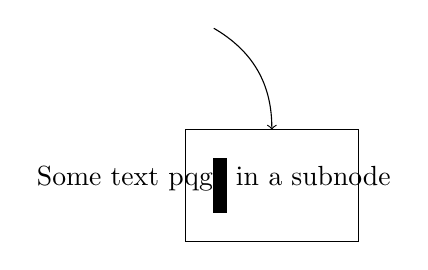
\begin{tikzpicture}[remember picture]
\node {Some \subnode[inner sep=10pt]{stuff}{text pqg\rule[-10pt]{5pt}{20pt}} in a subnode};
\draw[->] (0,2) to[bend left] (stuff.north);
\node[fit=(stuff),draw,inner sep=0pt] {};
\end{tikzpicture}

\newpage


\begin{lstlisting}[language=TeX,name=texcode,numbers=left,breakatwhitespace=true,breaklines=true]
\newcommand\balloon[4]{%
  \pgfmathtruncatemacro\firstline{%
    #3-1
  }%
  \iftikzmark{line-#2-\firstline-start}{%
    \iftikzmark{line-#2-#3-first}{%
      \xdef\blines{({pic cs:line-#2-\firstline-start} -| {pic           cs:line-#2-#3-first})}%
    }{%
      \iftikzmark{line-#2-#3-start}{%
        \xdef\blines{({pic cs:line-#2-\firstline-start} -| {pic             cs:line-#2-#3-start})}%
      }{%
        \xdef\blines{(pic cs:line-#2-\firstline-start)}%
      }%
    }%
  }{%
    \xdef\blines{}%
  }%
  \foreach \k in {#3,...,#4} {%
    \iftikzmark{line-#2-\k-first}{%
      \xdef\blines{\blines (pic cs:line-#2-\k-first) }
    }{}
    \iftikzmark{line-#2-\k-end}{%
      \xdef\blines{\blines (pic cs:line-#2-\k-end) }
    }{}
  }%
  \ifx\blines\empty
  \else
  \edef\temp{\noexpand\tikz[remember picture,overlay] \noexpand\node[fit={\blines},balloon] (#1) {};}%
\temp
  \fi
}
\end{lstlisting}

\begin{tikzpicture}[remember picture,overlay,>=stealth']
\draw[<-,ultra thick] (pic cs:line-texcode-1-end) +(1em,.7ex) -| +(2.5,1) node[above,comment,thin] {Command name};
\draw[<-,ultra thick] (pic cs:line-texcode-3-end) ++(1em,.7ex) -| +(5.8,1) node[above right,comment,thin] {Find previous line};
\draw[<-,ultra thick] (pic cs:line-texcode-5-end) ++(1em,.7ex) -| +(2.2,.5) node[above,comment,thin] {If previous line exists, add to the list};
\draw[<-,ultra thick] (pic cs:line-texcode-18-end) ++(1em,.7ex) -| +(2.2,.5) node[above,comment,thin] {Loop through rest of lines};
\draw[<-,ultra thick] (pic cs:line-texcode-28-end) ++(1em,.7ex) -| +(1,1.5) node[above,comment,thin] {Add a node covering all the lines};
\end{tikzpicture}

\newpage
\lipsum[6]

\vlstart\lipsum*[5]\vlend

\lipsum[7]

\newpage

\hlboxstart\lipsum*[4]\hlboxend

\hlstart\lipsum*[1]\hlend

\hlstart\lipsum*[2]\hlend

\fdstart\lipsum*[3]\fdend

\hlstart A not so long sentence\hlend

A rather longer \hlstart sentence that goes over one line and onto the next but not all that much further\hlend\ than that.

A rather longer sentence that goes over one line and onto the next but not all that much further than that.

\tikz[overlay,remember picture,ultra thick,red] \draw (pic cs:a) -- (pic cs:b);%
A\tikzmark{a} tikzmark

\lipsum[1-4]
\lipsum[4]
\lipsum*[4]
\tikzmark{b}%

\lipsum[1]
\tikz[overlay,remember picture,ultra thick,red] \draw (pic cs:a) -- (pic cs:b);

\newpage

\tikzset{
  next page=below,
}

\tikz[overlay,remember picture,ultra thick,red] \draw (pic cs:a) -- (pic cs:b);
\tikz[overlay,remember picture,ultra thick,red] \draw (0,0) -- (pic cs:d);

A\tikzmark{a} tikzmark \tikzmark{b}.

\lipsum[1-4]
\lipsum[4]
\tikzmark{c}%
\lipsum*[4]
\tikzmark{d}%

\lipsum[1]
\tikz[overlay,remember picture,ultra thick,red] \draw (0,0) -- (pic cs:d);


\end{document}

% Local Variables:
% tex-output-type: "pdf18"
% End:
%